\documentclass[11pt]{article}
\usepackage[margin=2.7cm]{geometry}
\usepackage{amsmath,amssymb}
\usepackage{graphicx}
\usepackage{booktabs}
\usepackage[hidelinks]{hyperref}

\newcommand{\Myr}{\,\mathrm{Myr}}
\newcommand{\pc}{\,\mathrm{pc}}
\newcommand{\kms}{\,\mathrm{km\,s^{-1}}}
\newcommand{\lam}{\lambda}

\title{WAKE: a visitation-statistics atlas of the solar neighbourhood ---\\
arrival statistics, an exclusion map, and a flyby network\\
on Gaia DR3 kinematics\\[1ex]
\large (Preprint --- English version; a Japanese version accompanies this record)}
\author{Yukie Maeda\thanks{Independent researcher. The roles of AI systems and
the complete verification protocol are disclosed in Appendix~B; this internal
verification is not a substitute for human peer review.}}
\date{August 2026}

\begin{document}
\maketitle

\begin{abstract}
\noindent Should we have been visited? We present the first calculation of
visitation statistics for the solar system on the \emph{observed} stellar
kinematics of the solar neighbourhood: arrival statistics of close stellar
passages on Gaia DR3 (56{,}286 stars with 6D phase-space data within 100 pc),
combined with settlement dynamics in the probe-based, entry-driven convention
of Carroll-Nellenback et al. Our contributions are three layers on one
catalogue. (1) \emph{Arrival statistics}: a completeness-corrected,
exposure-normalized encounter rate with explicitly declared accounting
conventions --- reconstructing the accounting of the two published rate camps
on our own data, we find their factor-of-two split is dominated by the
population that the completeness correction targets, not by data quality; we
also identify a third systematic mode (faint-end Gaia RVS radial-velocity
artifacts) that evades both value- and error-based quarantines and can
inflate encounter rates severalfold, and we introduce a tangential-velocity
consistency test to flag it. Our clean rate is
$\lam(1\pc)=4.5^{+4.0}_{-2.7}\Myr^{-1}$ for the FGK+early-M population.
(2) \emph{An exclusion map}: conditional statements of the form ``if the
settled fraction exceeds $f^*$, the solar system should have been visited
within the past 10\;Myr (silence rejected at 95\%)''; at the standard probe
range of 3.07\;pc we obtain $f^*=5.0\times10^{-3}$. A three-valued theorem
layer imports the survival theory proved in a companion mathematics paper
(DOI 10.5281/zenodo.21955413), separating where survival is
theorem-guaranteed, where the theorem is silent, and recording that no
extinction theorem exists for the full model anywhere. (3) \emph{A flyby
network}: on the time-varying graph of close passages, a propellant-minimal
visiting route exists at all times in the window, with a single-transfer
departure budget of $\Delta v\simeq5.8\kms$ --- a statistical property of the
network, not of any particular star. All statements are conditional
probability statements over a declared population; undecidable regions are
reported as undecidable. This is surveying, not proof.
\end{abstract}

\tableofcontents

%======================================================================
\section{Introduction}\label{sec:intro}

Should we have been visited? If settled systems exist in the Galaxy and
expand in the cheapest available channel --- slow, small, and old probes
launched at close stellar passages --- then the question of whether the solar
system has been reached is not a matter of speculation but of
\emph{measured kinematics}: which stars have passed within probe range, when,
and at what rate, given the selection function of the survey that observed
them. This paper computes those statistics on Gaia DR3 and overlays
settlement dynamics on them.

This is the third branch of a visitation-hypothesis research programme
(warp-class channels were treated in ASTROGATION, higher-dimensional
channels in TESSERA); the present branch is the sub-light channel, for which
the solar neighbourhood's real kinematics are the decisive input. Our claim
to novelty is deliberately narrow: \emph{the overlay of settlement dynamics
on real-catalogue encounter statistics}. The first layer alone --- encounter
statistics --- is a well-developed field \cite{bj18,bj22,gs01,fp26}; we treat
it as our verification bench, reproducing published anchors before adding
anything (Section~\ref{sec:prop}). The mathematical foundations of the
settlement-dynamics layer (survival and extinction theorems for contact
processes on ballistically moving points) were established in a companion
mathematics paper \cite{wakemath}; here we import only its assumptions map
and guarantees. Throughout, the discipline of the project constitution
applies: every output statement is a conditional probability statement over
a declared stellar population; regions where the data cannot decide are
reported as \emph{undecidable}, never silently filled; and the whole is
surveying, not proof.

%======================================================================
\section{Data, selection, and quarantine}\label{sec:data}

\subsection{Catalogue and completeness}
We use the Gaia DR3 six-dimensional sample within 100\;pc: 56{,}286 stars
with astrometry and radial velocities \cite{gaiadr3}. Selection is corrected
by inverse-probability weighting (IPW) over the DR3 RVS selection function
\cite{gaiaunlimited}, with a floor $s_{\rm floor}=0.05$: stars with selection
probability below the floor are not up-weighted but reported as an
\emph{undecidable population} (697 stars), so that the corrected population
is explicitly FGK and early-to-mid M. Late-M and fainter populations are
excluded from all rates and flagged as undecidable (a bounded-rate extension
is reserved but not used here).

\subsection{Five quarantine systems and a third failure mode}
\label{sec:bit5}
Individual-event claims are protected by quarantine flags: astrometric
quality, proper-motion signal-to-noise, extreme radial velocities
($|RV|>550\kms$, with a whitelist path for confirmed hypervelocity stars),
and a radial-velocity error cut ($\sigma_{RV}>20\kms$ excluded from
individual event judgements while still contributing to rates).

During the accounting cross-checks of Section~\ref{sec:arrival} we
identified a \emph{third} systematic mode that evades both the value-based
and the error-based quarantines: \textbf{faint-end RVS radial-velocity
artifacts} --- stars at $G\gtrsim14$ with $|RV|=150$--$900\kms$ but
disk-like tangential motion. Genuine halo stars show halo kinematics in
\emph{both} components; a disk-like tangential velocity with an extreme
radial velocity is the artifact signature (cf.\ the DR3 RV quality
guidance of \cite{katz23}). We therefore add quarantine bit~5
($G>13.5\wedge|RV|>150\kms$; 1{,}323 stars; threshold scanned over
$120/150/200\kms$ with a stable clean component), operated like the
hypervelocity bit: excluded from individual event judgements, rates
reported \emph{both ways} (clean and suspect-inclusive), manual review by
the tangential-velocity consistency test, and a rescue whitelist (empty
after review: every top suspect showed the artifact signature, e.g.\
$RV=-790\kms$ with $v_{\rm tan}=18\kms$). Left unquarantined, this
population would inflate the sub-parsec encounter rate by a factor of
$\sim$7 (Section~\ref{sec:arrival}); we flag this as a general
methodological caution for DR3-based encounter studies.

%======================================================================
\section{Propagation and verification}\label{sec:prop}

Orbits are propagated in an axisymmetric Galactic potential
(MWPotential2014-class) by direct numerical integration; an independent
epicyclic analytic path serves as the formulation-independence counter-path
(gate G2). Verification anchors (gate G3) reproduce published encounters
before any new statistics are claimed: the Scholz-star flyby
\cite{mamajek15,dupuy19}, GJ~710 (our value $1.294\Myr$, $0.0503\pc$,
in agreement with \cite{dlfm22}; the published-value split among DR3
analyses is documented neutrally in Appendix~A), and the encounter-frequency
anchor \cite{bj18}. A dual-potential audit (McMillan17 \cite{mcmillan17}
via a spline tabulation whose interpolation error is itself audited,
max $3.7\times10^{-5}$ relative) bounds potential systematics; where the
two-potential difference exceeds a star's measurement uncertainty at far
epochs, the star's \emph{effective horizon} is shortened
(``$t_{\rm pot}$'', a third horizon component), so that model uncertainty is
treated exactly like measurement uncertainty: as undecidability, not as
noise to be averaged.

Each star carries an \emph{individual horizon} $t_h$: the epoch beyond which
its position uncertainty (dominated by the radial-velocity error,
$1\kms\approx1\pc\Myr^{-1}$) exceeds half the probe range. Statistics are
computed in the \emph{control region} $|t_{\rm ph}|\le t_h$; events beyond
horizons form the undecidable shadow visible in
Figure~\ref{fig:lambdat} --- the measured ``evidence horizon'' of the
catalogue. Two implementation defects found and fixed by the G2 gate during
this work (a parabolic-refinement coefficient and a sharp-minimum
breakdown, repaired by exact $d^2$-interpolation; all G3 anchors re-passed)
are disclosed in Appendix~B.

\begin{figure}[t]\centering
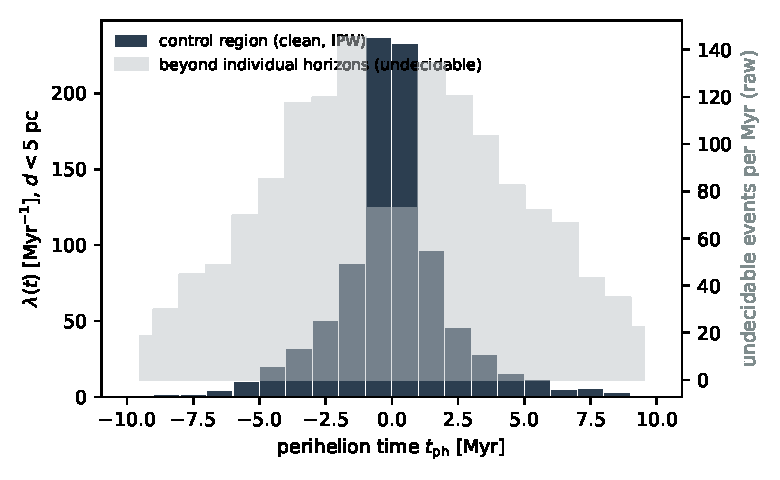
\includegraphics[width=.7\textwidth]{figs/fig1_lambda_t.pdf}
\caption{Exposure-normalized arrival rate $\lam(t)$ within 5\;pc for the
clean population (bars), with the undecidable shadow of events beyond
individual horizons (gray). The envelope is the measured evidence horizon of
Gaia DR3: rates are only claimable where the catalogue can support them.
Reproduce: \texttt{python3 src/wake\_p5/paper\_figs\_main.py}.}
\label{fig:lambdat}
\end{figure}

%======================================================================
\section{Arrival statistics and the accounting of encounter rates}
\label{sec:arrival}

\subsection{Exposure accounting}
A rate is a count divided by an exposure, and the choice of exposure is a
convention that must be declared. We normalize each star's contribution by
its own effective exposure $2\min(T,t_h)$ within the control region. A
naive uniform window ($1/2T$) dilutes the rate as $T$ grows past typical
horizons; our own first-look value of $11.7\Myr^{-1}$ at 1\;pc arose from
exactly that convention (horizon-ignored, uniform-window) and is
reproduced exactly under it --- a downward-biased accounting, not a
different sky. The exposure-normalized clean rates are
\[
\lam(1\pc)=4.49\;[1.78,8.50]\Myr^{-1},\quad
\lam(2\pc)=27.5\Myr^{-1},\quad
\lam(5\pc)=137.3\Myr^{-1}
\]
(95\% star-bootstrap interval at 1\;pc; population: FGK+early-M,
IPW-corrected; suspect-inclusive values are co-reported in the catalogue).
The rate scaling departs from the geometric $d^2$ law ($6.1\times$ from 1
to 2\;pc, $5.0\times$ from 2 to 5\;pc), reflecting heavy-tailed,
few-star-dominated contributions and the distance structure of the IPW
weights; the $d^2$-law tests of Section~\ref{sec:prop} live in the
BJ-convention reconstruction, a different accounting.

\subsection{Three conventions on one data set}
The two published 1-pc rate camps --- $19.7\pm2.2\Myr^{-1}$ \cite{bj18} and
$10.6\pm4.5\Myr^{-1}$ \cite{fp26} --- use different accounting conventions
(window, exposure, completeness target, and population). We reconstructed
both conventions from the published texts (the reconstruction limits ---
five points for \cite{bj18}, seven for \cite{fp26} that could not be
determined from the texts --- are listed neutrally in Appendix~A) and
applied all three to our single data set:

\begin{center}
\begin{tabular}{lll}
\toprule
Convention (on our data) & $\lam(1\pc)$ [$\Myr^{-1}$] & Published \\
\midrule
Ours (control region, IPW, per-star exposure) & $4.5^{+4.0}_{-2.7}$ & --- \\
BJ+18 reconstruction ($G\le12.5$ subset) & $23.7\pm2.6$ & $19.7\pm2.2$ \\
FP26 reconstruction (discrete, reliability cut) & $21.3$ & $10.6\pm4.5$ \\
\bottomrule
\end{tabular}
\end{center}

The BJ-convention value is reproduced on clean DR3 data --- so residual
spurious astrometry is unlikely to be the main driver of the published
split. The remaining FP26 gap closes when the faint-end RV artifacts of
Section~\ref{sec:bit5} are excluded (bright-only discrete counting gives
$\simeq7.6$, matching their solar value of $9.1$). Based on this
reconstruction, the split is dominated by the \emph{population that the
completeness correction targets}: \cite{bj18} corrects to the full mock
stellar population, \cite{fp26} does not correct beyond a window factor.
Consistently, a two-ledger check on our own data --- correcting by
per-star exposure and IPW (denominator ledger) versus by a mock-based
$C(t,d)$ completeness map (numerator ledger, Appendix~C) --- yields a
measured \emph{population bridge} of $5.3\times$ between the FGK+early-M
and full-population rates, compared with the $\sim9\times$ implied by the
mock extrapolation of \cite{bj18}; the difference is a quantitative basis
for critiquing mock-based completeness corrections.

\subsection{Arrival catalogue and structure}
The arrival-event catalogue (2{,}197 stars with median perihelion within
5\;pc inside $|t|\le13\Myr$) reproduces the well-known close passages ---
HD~7977 ($0.037\pc$, $-2.76\Myr$), GJ~710 ($0.052\pc$, $+1.29\Myr$) --- and
carries all quarantine, horizon, and both-ways rate metadata. The
time-resolved rate $\lam(t)$ shows no kinematically coherent clumps (all
apparent clumps are single-star dominated; pairwise $\Delta UVW\ge45\kms$),
and the small approaching-vs-receding excess ($+2.1\%$ relative) is the
textbook solar-apex dipole (approaching fraction $75.4\%$ toward the apex
hemisphere vs.\ $24.1\%$ away); after subtracting the sample mean-field
reflex it reduces to $+0.78\%$ ($1.9\sigma$) --- consistent with no spatial
structure.

%======================================================================
\section{The exclusion map}\label{sec:map}

\subsection{Definition}
The map's conditional statement is defined by a Poisson visit count:
\begin{equation}
N_{\rm vis} = f\cdot\frac{\langle \hat p\rangle}{f}\cdot\lam(R)\cdot
T_{\rm eff},\qquad
N_{\rm vis}\ge3\;\Longleftrightarrow\;P(\ge1\ \text{visit})\ge95\%,
\label{eq:fstar}
\end{equation}
with $T_{\rm eff}=\max(0,\,10\Myr-R/v_p)$ the support-limited retrospective
window (probe travel time deducted), $f$ the settled fraction,
$\langle\hat p\rangle/f$ the mark-field factor (unity for the constant
field; evaluated on the real arrival kinematics for the front family), and
$\lam(R)$ the clean-population rate interpolated between measured anchors
(below 1\;pc: $d^2$ extrapolation, flagged; above 5\;pc: undecidable).
The clean rate is a \emph{lower bound} on the physical encounter rate
(probes do not obey Gaia's selection function), so the
``should-have-been-visited'' region is conservatively small; a
population-bridge reference layer ($\times5.3$, model-explicit) and the
suspect-inclusive layer are co-reported.

\begin{figure}[t]\centering
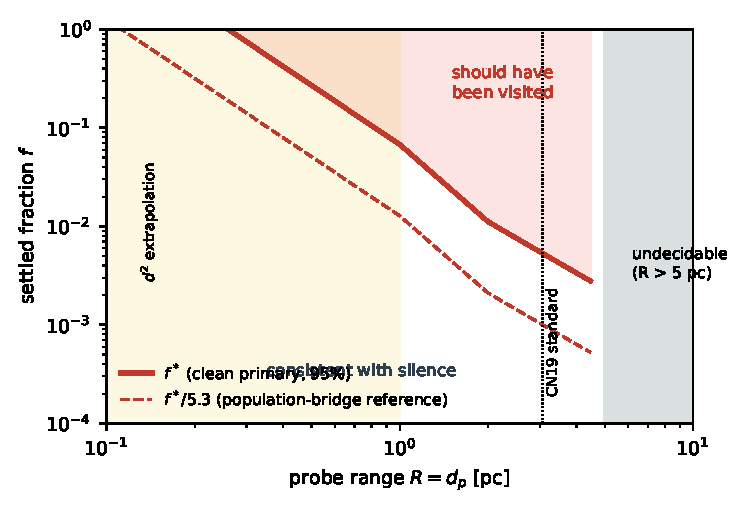
\includegraphics[width=.72\textwidth]{figs/fig2_exclusion_map.pdf}
\caption{The exclusion map in the $(R,f)$ plane at $v_p=10\kms$ (constant
mark field). Above $f^*$ (solid), silence is rejected at 95\% for the
declared population; the dashed line is the population-bridge reference.
Gray: undecidable ($R>5\pc$); yellow band: $d^2$-extrapolated. At the
standard probe range $R=3.07\pc$: $f^*=5.0\times10^{-3}$.}
\label{fig:map}
\end{figure}

At the standard probe range of \cite{cn19} ($R=3.07\pc$),
\[
\boxed{f^* = 5.0\times10^{-3}}
\]
--- \emph{if more than half a percent of systems in the declared population
are settled (and launch on entry), the solar system should have been visited
within the past 10\;Myr.} At $R=1\pc$, $f^*=6.8\times10^{-2}$
(Figure~\ref{fig:map}); boundary uncertainty follows the rate interval
($\times0.53$--$\times2.52$).

\subsection{The three-valued theorem layer}\label{sec:theorem}
The settlement-dynamics layer imports the survival theory of
\cite{wakemath} with its assumptions, not beyond them. The assumptions map
(mixing number $K_{\rm mix}=w_1T_s/R\ge20$; bounded relative density
$\bar\Lambda\le4$ on a speed shell, which the isotropized DR3 distribution
satisfies non-trivially at $\bar\Lambda=3.3$--$3.6$) yields a
\textbf{three-valued legend}: (i) \emph{C2-guaranteed} (assumptions hold and
the numerical threshold is exceeded), (ii) \emph{theorem-silent}
(assumptions fail --- notably the \emph{entire} standard scan domain of
\cite{cn19}, $R=3.07\pc$ with $T_s=0.1$--$1\Myr$, is theorem-silent;
guarantees open only at $T_s\gtrsim3\Myr$), and (iii) the reminder that
\emph{no extinction theorem exists for the full model anywhere} (the
companion paper proves the SIR-type bound does not extend), so
``settlement impossible'' is nowhere theorem-backed. The asymmetry is
physical: for short-lived settlements the mathematics is silent; the longer
settlements live, the more strongly silence constrains them. Where the
theorem is silent the only judgement material is the numerical threshold,
which we \emph{re-calibrated on the measured kinematics}: the survival
threshold shifts from the isotropic calibration $m\approx1.0$--$1.3$ to
$m\approx1.5$--$2.0$ (Figure~\ref{fig:e9}) --- real anisotropic kinematics
are \emph{harsher} to settlement fronts than the isotropic approximation,
which gives the pure-isotropy open problem of \cite{wakemath} an
observational demand.

\begin{figure}[t]\centering
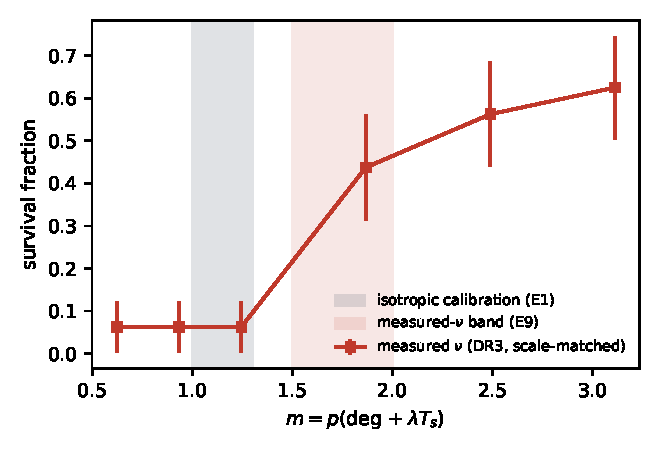
\includegraphics[width=.55\textwidth]{figs/fig5_e9.pdf}
\caption{Survival threshold on measured DR3 kinematics (scale-matched to
the isotropic calibration): the threshold band shifts upward by
$\sim1.5\times$. The exclusion map's guarantee layer uses the conservative
edge ($m>2.0$).}
\label{fig:e9}
\end{figure}

\subsection{Front-direction sensitivity}
For the front-family mark field, the direction average over two priors
(uniform sphere vs.\ galactocentric bias) shifts the map by only $2.5\%$
--- prior-robust. The \emph{per-direction} spread is large ($52\%$):
arrivals are apex-concentrated, so a settlement front's effectiveness
depends on its direction relative to the solar apex --- a direction
dependence we report as a finding connecting to the settlement-direction
discussion of \cite{wright21}.

%======================================================================
\section{The flyby network}\label{sec:flyby}

On the time-varying graph of clean solar passages (646 nodes within
horizons, perihelion states extracted by the numerical propagator), we ask
the constitution's third-layer question: what is the propellant-minimal
visiting route? A visitor riding any passing star may transfer, by one
ballistic cruise leg, to a star whose perihelion is arbitrarily deep in the
solar system. The minimal single-transfer departure budget is
\[
\Delta v \simeq 5.8\kms
\]
--- and this is a \emph{statistical property of the network}, not of a
particular star: over the error-MC ensemble the route exists in 100\% of
draws with median $5.7$--$5.9\kms$ (departure charged entirely to
propellant --- co-moving riders cannot use flybys to accelerate --- so the
budget is an upper bound). Direct passages within $0.1\pc$ in the window
are HD~7977 and GJ~710, matching the known record. The graph estimate is
validated by a formulation-independent counter-path: Jacobian shooting in
the full potential converges to sub-0.1-mpc misses and shifts the transfer
budget by at most $0.19\kms$ (tidal terms are subdominant).
Multi-leg optimization, full ensemble re-extraction, and real stellar
masses are reserved for v1.1 of the network file.

\begin{figure}[t]\centering
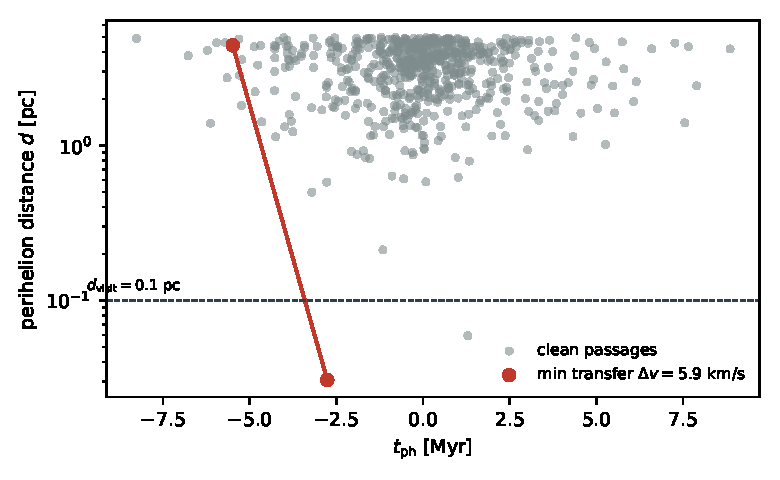
\includegraphics[width=.68\textwidth]{figs/fig3_flyby.pdf}
\caption{The flyby network's node set (clean passages; perihelion distance
vs.\ time) and the minimal single-transfer route into $d\le0.1\pc$.}
\label{fig:flyby}
\end{figure}

%======================================================================
\section{Discussion}\label{sec:disc}

\textbf{The philosophy of undecidability.} The atlas's reliability rests on
an asymmetry principle --- prefer undecidable over falsely decidable ---
implemented in three mechanisms: individual horizons with three components
(measurement growth, potential-model divergence, budget-type truncation),
five quarantine systems with both-ways reporting, and the three-valued
theorem layer. Nothing in the map is painted by silent extrapolation.

\textbf{Limitations.} The theorem layer judges under an isotropized
approximation of the measured velocity distribution (the real distribution
is anisotropic; E9 quantifies the direction of the error). The flyby
network assumes solar-mass deflectors and single transfers. The $d^2$
extrapolation below 1\;pc and everything above 5\;pc are flagged. The
population is FGK+early-M; late-M visitation channels are undecidable here
(a bounded-rate extension is reserved).

\textbf{Comparisons with published values} rest on our reconstruction of
published accounting conventions; the points that could not be determined
from the texts are listed openly in Appendix~A. DR4 replacement is designed
in from the start (the catalogue is a swappable data layer).

%======================================================================
\section{Conclusions}\label{sec:concl}

On the observed kinematics of the solar neighbourhood, with a declared
population and declared accounting: (1) the clean arrival rate at 1\;pc is
$4.5^{+4.0}_{-2.7}\Myr^{-1}$, and the published factor-of-two split is
dominated by completeness-target population choices, not data quality;
(2) if more than $0.5\%$ of systems (standard probe range) are settled, the
solar system should have been visited within the past 10\;Myr --- silence is
informative at 95\% above that line, and the mathematics guarantees
survival of settlement processes only for long-lived settlements, so
silence constrains long-lived settlement most strongly; (3) a
propellant-minimal visiting route through the real stellar traffic exists
at $\Delta v\simeq5.8\kms$ at all times. Methodologically we contribute the
exposure-accounting analysis, the faint-end RV artifact quarantine with its
tangential-velocity test, and the two-ledger completeness check with its
measured population bridge. The atlas is surveying, not proof --- but it
turns the visitation question into numbers that Gaia DR4 can sharpen.

%======================================================================
\appendix

\section{GJ 710, published-value splits, and reconstruction limits}
\label{app:gj710}
[GJ~710 perihelion values across DR2/DR3 analyses; our reproduction
($1.294\Myr$, $0.0503\pc$) agrees with \cite{dlfm22}; a unit-conversion
hypothesis for one published time value is stated neutrally
(our $1.294\Myr$ expressed in pc/(km/s) units equals $1.3234$, coinciding
with the published $1.324\pm0.026$ to 0.1\%). The full accounting
comparison table for \cite{bj18} and \cite{fp26}, with the twelve points
that could not be determined from the published texts, is reproduced here
from the repository records; these lists disclose the limits of our
reconstruction.]

\section{Method record and AI disclosure}\label{app:method}
[Complete verification protocol: claim-driven falsification against an
independent simulation device; machine certification of geometric
constants; error ledger including the two propagation-refinement defects
found by gate G2 and the ``agreeing numbers are the ones to distrust''
episode (two mutually confirming rate values, $11.7$ and $20.3$, were both
wrong for different reasons and were caught by convention identification
and engine re-verification). Roles of AI systems (Claude Code, model Claude
Fable 5) as executor under human arbitration; steering-intervention log
empty; this internal verification is not a substitute for human peer
review.]

\section{Completeness-map bin width as a hidden regularizer}
\label{app:binwidth}
[The mock-based $C(t,d)$ completeness map's bin width acts as a hidden
regularization parameter: the reconstructed BJ-convention rate scans
non-monotonically ($46.5\to23.7\to20.4\to27.1\to20.7\Myr^{-1}$ for
$\Delta t=0.5\to3.0\Myr$; Figure~\ref{fig:binwidth}) --- fine bins diverge
through empty-cell $1/C$ weights, coarse bins alias. We adopt
$(\Delta t,\Delta d)=(1.5\Myr,0.75\pc)$ with a $\pm15\%$ grid-systematic
band, and co-report the canonical $(1.0,0.5)$ value.]

\begin{figure}[t]\centering
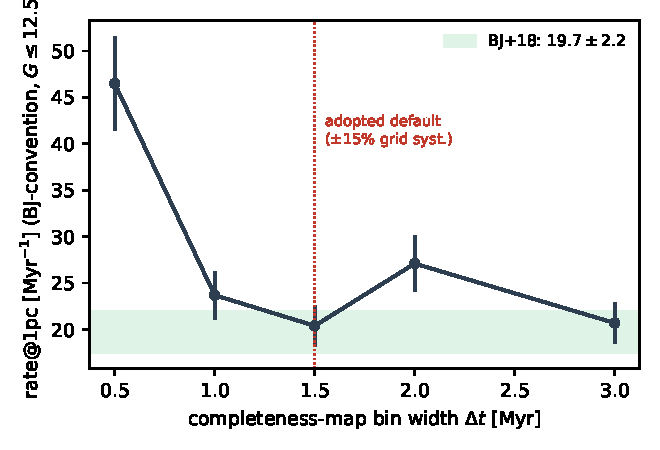
\includegraphics[width=.5\textwidth]{figs/fig4_binwidth.pdf}
\caption{Bin-width scan of the mock-completeness rate reconstruction: a
hidden regularization parameter, disclosed.}
\label{fig:binwidth}
\end{figure}

\section{Reproducibility and data release}\label{app:release}
[The public data set: \texttt{arrival\_catalog\_v1.json},
\texttt{exclusion\_map\_v1.json} (v1.0.1),
\texttt{flyby\_network\_v1.json}, with a SHA-256 manifest; regeneration
commands for every figure and table; the browser simulator reads exactly
these files (additive-compatibility schema principle). This appendix is the
paper-side anchor of the three-artifact consistency audit (paper,
data/maps, simulator).]

\bibliographystyle{plain}
\bibliography{wake_refs}

\end{document}
